本章将会介绍本文关于API知识抽取领域的研究背景、国内外研究现状、研究的目的及意义,以及本文相对国内外已有的工作的创新之处和本文的贡献。最后,本章还会介绍本文的整体篇章结构。

\section{研究背景}
在软件开发的过程中,软件开发者们遇到的大部分编程任务通常都需要使用由编程语言和第三方库所提供的各种API(Application Programming Interfaces)来完成实现。在开发过程中,程序员们一般会通过阅读API文档来学习一个API\cite{DBLP:conf/sigsoft/FucciMM19}\cite{DBLP:conf/icsm/LiLSXPLZ18}。一个API文档通常带有和功能、结构相关的知识,但缺少与概念和使用目的相关的信息\cite{DBLP:conf/se/MaalejR14}。而程序员在学习如何使用一个API时,最常见的困难就是API文档中信息的缺失,特别是与API的设计、基本原理、使用场景和代码示例相关的信息的缺失\cite{DBLP:journals/ese/RobillardD11}\cite{DBLP:journals/software/Robillard09}\cite{DBLP:journals/chinaf/FanYWYW21}\cite{DBLP:journals/tse/ZhangJRZH21}。

因此,尽管大部分编程语言及第三方库都提供了对应的API文档,但是这些API文档并不能完全解决程序员的需求\cite{DBLP:journals/tse/ZhangJRZH21}\cite{DBLP:journals/corr/abs-1907-09807}。程序员更经常遇到的场景是只有一个编程任务的需求,而不知道需要使用到哪个API,或者在使用某个API时遇到了程序报错,而不知道如何去解决这个API带来的错误\cite{DBLP:conf/kbse/HuangXXLW18}\cite{DBLP:conf/sigsoft/SadowskiSE15}\cite{DBLP:journals/ese/WuWBI19},这种场景下,API文档通常很难对开发者有所帮助。当API文档不能解决程序员的问题时,程序员们通常使用搜索引擎来查询相关信息。最常搜索到的解决方案来自于Stack Overflow\cite{DBLP:conf/iwpc/ZhouXLTW14}。Stack Overflow\footnote{https://stackoverflow.com/}是一个程序开发领域的知识问答网站,网站允许注册用户提出或回答问题,自2008年以来,Stack Overflow已经为用户提供了451亿次帮助,每个月浏览量超过一亿次。在API文档不能完全解决开发者的难题时,Stack Overflow上的回答往往会成为API文档的补充。因此,在现代软件开发中,Stack Overflow已经成为了一个由所有用户众包构建而成的软件知识库\cite{DBLP:conf/sac/YeXLK16}\cite{王海2017社交化软件开发问答中的交互过程研究}。Stack Overflow涵盖了各种在软件开发过程中遇到的问题与解决方案,在这些问答中包括了许多与API相关的问题与答案。在这些问题与回答中,提问者与回答者通常会讨论与API相关的许多知识,包括关于API的调用方法、关于API的特性、关于API底层实现的逻辑或者API的使用场景等\cite{DBLP:conf/icalt/VenigallaLAC19}\cite{DBLP:journals/access/ZhangJRC18}\cite{DBLP:conf/wcre/AhasanuzzamanAR18}\cite{朱子骁2018基于}。

然而,这些有用的知识散落在Stack Overflow网站的各个帖子中,程序员在使用Stack Overflow进行搜索时,需要阅读它返回的大量帖子,并从中找到对自己有帮助的信息。由于如今问答型网站数据的大量增长,这个查询的过程可能会非常耗费精力\cite{DBLP:conf/sigsoft/CaiWXH00X19}\cite{和晓健2019基于实体识别的软件开发问答网站中的}。因此,软件工程领域的许多国内外学者都开始针对Stack Overflow中的API知识的抽取展开了研究,提出了许多方法从Stack Overflow中抽取出散落在庞大的帖子数据中的API知识并进行汇总分类。根据API知识抽取的方法、来源以及抽取目标不同,这一方面的研究也分成了不同的分支。虽然现有的这些研究在某些方面能够有较好的效果,但仍然在其他方面有所不足。

由于机器学习方法在自然语言处理上表现良好,有学者提出了基于机器学习方法从Stack Overflow的帖子中抽取出API知识并对API文档进行补充。Treude等人\cite{DBLP:conf/icse/TreudeR16}提出了一种被称作SISE的机器学习方法,它将Stack Overflow上文本包含的大量信息作为文本特征输入,包括句子本身、句子的语言模式、句子的词性标签、句子来源帖子的问题与回答、作者名以及句子与目标API文档的句子相似度。作者先是人工标注了1574个句子作为训练集,训练得到一个识别模型,然后从Stack Overflow文本中自动识别出符合特征要求的句子作为补充到API文档中的备选对象。SISE方法在标注得到的句子中实现了64\%的精确度和70\%的覆盖率。Treude等人的方法虽然能够得到不错的效果,但SISE方法仅仅是从Stack Overflow中抽取出与API的观点有关的句子,并没有对这些API观点进行结构化的分析,也没有对观点进行分类。并且这项工作中用于训练SISE模型的标注句子均来自Stack Overflow上的热门帖子,这让SISE模型具有了时效性,其中涉及的API都是当前版本的API,随着软件开发库的迭代更新,使用之前版本的句子训练出来的模型的预测准确性可能会下降。

Souza等人\cite{DBLP:journals/infsof/SouzaCDPRM19}提出了一种基于LDA(Latent Dirichlet Allocation)主题提取算法的编程指导文档生成方法,从Stack Overflow的帖子中找到那些与特定编程任务以及API相关的问答对,然后使用LDA主题提取算法将这些问答对的主题提取出来,并将这些主题作为章节,将带有同一主题的问答对归类到一起,以此生成一个基于编程任务的编程指导文档。Souza等人的工作还对编程指导文档的设计做出了贡献,并将生成的编程指导文档视为API文档的补充,用户可以通过查阅编程指导文档来找到与具体编程任务相关的Stack Overflow帖子。这项工作是较为粗粒度的,直接将Stack Overflow帖子作为分类方法中的最小分类单位,用户在使用编程指导文档辅助开发的时候,仍然需要阅读文档中的整个问答帖子。

Uddin等人\cite{DBLP:journals/tse/UddinK21}提出了一种基于情感分析的知识抽取算法,用于从Stack Overflow中自动地将关于API的观点抽取出来并分类。该方法基于Novielli等人\cite{DBLP:conf/sigsoft/NovielliCL15}对Stack Overflow上的句子情感的研究和Hu等人\cite{DBLP:conf/kdd/HuL04}提出的主导情绪取向研究(DSO),结合前人的研究提出了一种用于检测API观点情感的算法Opiner。该方法首先对Stack Overflow网站上关于API的讨论句子中的观点设计了11个不同的分类,并创建了一个基准数据集,人工标注出数据集句子中的观点,接着使用基于机器学习的方法抽取出带有API观点的句子,并使用Opiner算法从中抽取出带有情感的API观点并进行分类,最后将这些抽取出来的API观点与API实体相关联。Uddin等人的这项工作是目前本领域较为优秀的API知识方法,抽取出来的API知识质量较高,覆盖面较广,但也有其不足之处。由于Uddin等人设计的API知识分类太多,导致方法中的API观点分类准确率只有0.502,这会影响到抽取出来的API知识的数量。

以上工作在API知识抽取领域都取得了一定的突破,能够在一些特定场景下抽取出高质量的API知识,但在抽取出来的API知识的粒度、抽取方法的性能等方面则有着一定的短板。

\section{研究目的及意义}
现代软件开发要求开发者们复用由编程语言和第三方库提供的API来完成编程任务。在学习一个API如何使用时,常用的方法就是查阅API的官方文档。有研究表明,程序员在学习如何使用一个API时,最常见的困难就是API文档中的信息并不能满足软件开发的要求\cite{DBLP:journals/ese/RobillardD11}。通常,API文档只提供了与功能和输入输出结构相关的知识,并不会涉及到API的设计、具体实现、使用场景和代码示例等方面。而在API文档中的知识不足以满足开发者的需求时,人们通常会转向Stack Overflow上寻求帮助。Stack Overflow上有许多帖子里包含了与API相关的讨论,其中包含着大量高质量的API知识。但这些知识分布在Stack Overflow的各个帖子中,这也为程序员使用Stack Overflow解决问题造成了一定的困扰。综上所述,从Stack Overflow的帖子中抽取出API相关的知识并进行汇总,能够对API文档起到补充的作用,这对开发者是非常有价值的。

\section{主要工作和创新点}
如前文所简单介绍的,国内外有许多学者在API知识抽取这一领域完成了巨大的突破,提出了许多行之有效的方法,用于从给定的语料中抽取出API知识。但是这些工作也有着它们的不足之处。如Treude等人\cite{DBLP:conf/icse/TreudeR16}的工作仅仅是将与API知识相关的句子抽取出来,并没有对其进行结构化的分析以及对知识的分类;Souza等人\cite{DBLP:journals/infsof/SouzaCDPRM19}的工作得到的API知识以帖子为单位,知识粒度较大,用户仍需花费精力对抽取出来的知识进行理解消化;而Uddin等人\cite{DBLP:journals/tse/UddinK21}的工作对API知识的分类粒度过低,以至于影响了知识抽取的整体性能。

本文提出了一种基于自举思想的API描述性知识抽取方法,结合了机器学习分类方法和基于规则的知识抽取方法,并设计了与API描述性知识相关的概念结构,从广泛分布在Stack Overflow帖子里的API描述性知识句子中迭代地抽取出API描述性知识,选择了合适的知识分类粒度将抽取出来的知识根据组成元素自动分类,构建成一个API描述性知识图谱,并基于知识图谱实现了一个API描述性知识汇总应用。

本文的主要贡献如下:
\begin{itemize}
    \item 设计了一个用于描述API描述性知识的概念模型。
    \item 提出了一种基于自举思想的API描述性知识抽取方法,该方法结合了自顶向下和自底向上的知识抽取方法,能够迭代地在Stack Overflow帖子中抽取API描述性知识。
    \item 对抽取出来的API描述性知识汇总,构建了一个API描述性知识图谱,并基于知识图谱实现了一个知识汇总应用,用于补充API文档。
    \item 通过设计实验,对本文提出的方法进行验证,评估了本文方法流程的有效性,抽取得到的API描述性知识的有效性以及与API文档的互补性。
\end{itemize}

\section{篇章结构}
本文将围绕基于软件开发问答网站的API知识抽取方法研究与实现进行六个章节的介绍。

第一章,引言。本章主要介绍了基于软件开发问答网站的API知识抽取方法的研究背景以及研究意义和目的,并在仔细了解国内外与该课题相关的研究工作后对其他人的工作进行总结。本章的最后部分还阐明了本文的主要贡献以及在研究工作中所使用的创新技术。

第二章,背景知识及相关技术。本章介绍了目前国内外学者对API文档和软件开发问答网站Stack Overflow的研究,以及国内外学者对基于Stack Overflow的API知识抽取的相关研究。最后,本章还会介绍在本文中所使用到的相关技术以及自然语言处理工具。

第三章,方法概述。本章会对本文所设计的API描述性知识抽取方法进行详细的介绍。本章首先会介绍本文提出的方法的流程概览,然后介绍本文定义的API描述性知识概念模型。接着,本章还会给出一个具体的运行示例,用于帮助读者梳理整个抽取方法的流程。最后,本章会将抽取方法中的每一个步骤都进行详尽地介绍,包括API描述性知识句子的识别,基于概念变异的API描述性知识实例抽取,基于语言模式变异的API描述性知识元组抽取,以及API描述性知识图谱的构建。

第四章,系统的设计和实现。本章将会阐述上一章中介绍的API描述性抽取系统的具体实现,包括语料库生成模块,抽取主体模块以及知识图谱构建模块的设计与实现。本章的最后还介绍了基于API描述性知识图谱实现的知识汇总应用的设计与实现。

第五章,实验评估。本章将对本文提出的API描述性知识抽取方法以及抽取得到的API描述性知识质量进行评估,并对实验结果进行验证和分析,根据实验结果进行方法有效性与有效性威胁的总结。

第六章,总结与展望。本章会对本文提出的API描述性知识抽取方法进行总结,结合上一章中的实验结果分析以及有效性威胁分析,对未来的工作进行展望,规划未来的工作。



% 测试参考文献~\cite{ASE10Rule}。
% 图片示例\ref{fig:fig1}

% \begin{figure}[htb]
%     \centering
%     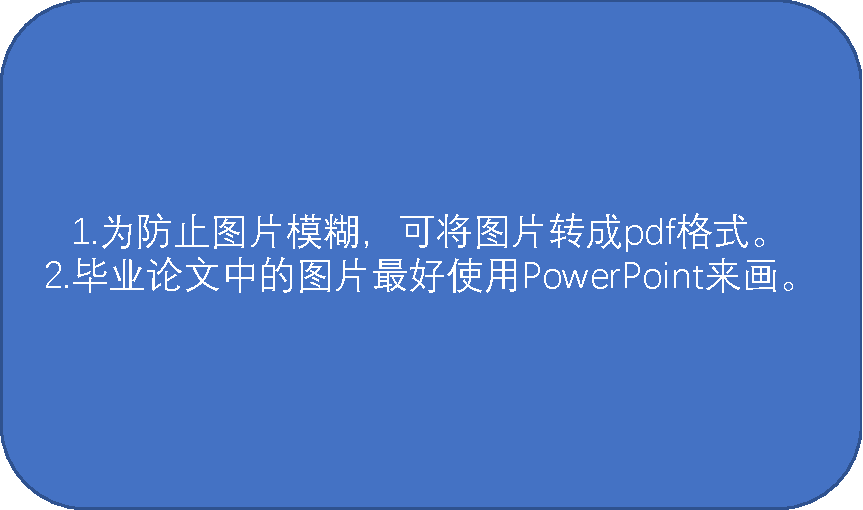
\includegraphics[width=\textwidth]{image/fig1.pdf}
%     \caption{代码示例的抽象语法树} 
%     \label{fig:fig1} 
% \end{figure}